\section{Gradient saliency and attribution maps}
\label{sec2}

Activation maps was the first step towards explaining the convolutional networks through inspection. For a given input sample (image), the response of each convolutional filter is recorded and plotted.

This method has several limitations:
\begin{itemize}
    \item The number of convolution filters of these networks is very large even for simple networks like LeNet (1-5)
    \item There is no visualization of the interactions between the layers. A small contribution on a given layer might be amplified by following layer and vice-versa
    \item After the 2\textsuperscript{nd} hidden layer it is very difficult to provide interpretation to what is seen
\end{itemize}

Many techniques have been developed from the 2000's to provide views on the networks internal that are human understandable. These techniques start from the feature space of a layer or a unit within a layer and apply an operation similar to a projection back to the original image space.

Since the original paper of \cite{Erhan2009}, many variations of the Saliency maps have been issued. Most of them are based on the gradient of the image.

The following contributions have been listed:
\begin{itemize}
    \item Deconvolution networks by \cite{Zeiler2013} from a convolutional unit within the network, the computation is reversed for each upstream convolution until the input of the network. Non linear units like activations and pulling are approximated
    \item Saliency maps (genuine) by \cite{Simonyan2014}, output of a layer or a unit is maximized by performing gradient ascent
    \item Gradient integral over a path by \cite{Sundararajan2017} in which input image is multiplied by the integrated gradient over a path from a baseline image (see below) to the observed activation. 
    \item Activation differences \cite{Shrikumar2017}, the contributions are evaluated over a full activation delta from the baseline image. Goal is to avoid null gradients that would cancel contributions in original saliency maps
\end{itemize}

All these techniques are evaluated in \cite{Ancona2018}. Following paragraphs are detailed reviews for each of these.

\subsection{Baseline input}

The latest techniques cited above are calculating the saliency starting from a baseline input to the network. As explained in \cite{Shrikumar2017} paragraph 3.3 and  \cite{Sundararajan2017} paragraph 5, there is no "one fits all" solution but for images it is often the neutral black or grey image.

Another solution is to select a reference image in order to detect the required changes to modify the activation of some unit or the classification change at the output. This is more like a perturbation as seen in the Adversarial networks see \ref{sec3}.

In the following, the actual test sample (image) is referred to as \(x = (x_1, ..., x_n)\), and the baseline is \(\tilde{x} = (\tilde{x_1}, ..., \tilde{x_n})\). The activation of the neuron unit of interest (or the final classification if observing the full network) is \(t\) for the sample, and \(\tilde{t}\) for the baseline. 

The differences are also defined as: 

\[ \Delta_{x_i} = x_i - \tilde{x_i}, \Delta_{t} = t - \tilde{t} \]

\subsection{Deconvolution networks}
\cite{Zeiler2013}

Deconvolution networks (DeconvNets, \cite{Zeiler2011}) were developed as an architecture similar to an auto-encoder. In \cite{Zeiler2013}, the DeconvNet is used as a tool to compute attribution to a given layer output (feature space) from the pixels of the image space.

It means reverting all operations of the convolutional network by applying the bijection function or an approximation:
\begin{itemize}
    \item Convolutional filters are flipped into the reverse or transpose filters
    \item Activation functions (ReLU) are approximated by the same rectifier function
    \item Maxpooling is approximated by an attribution to the input pixel that was selected in the pooling, using knowledge of the forward operation.
\end{itemize}

\begin{figure}[H]
    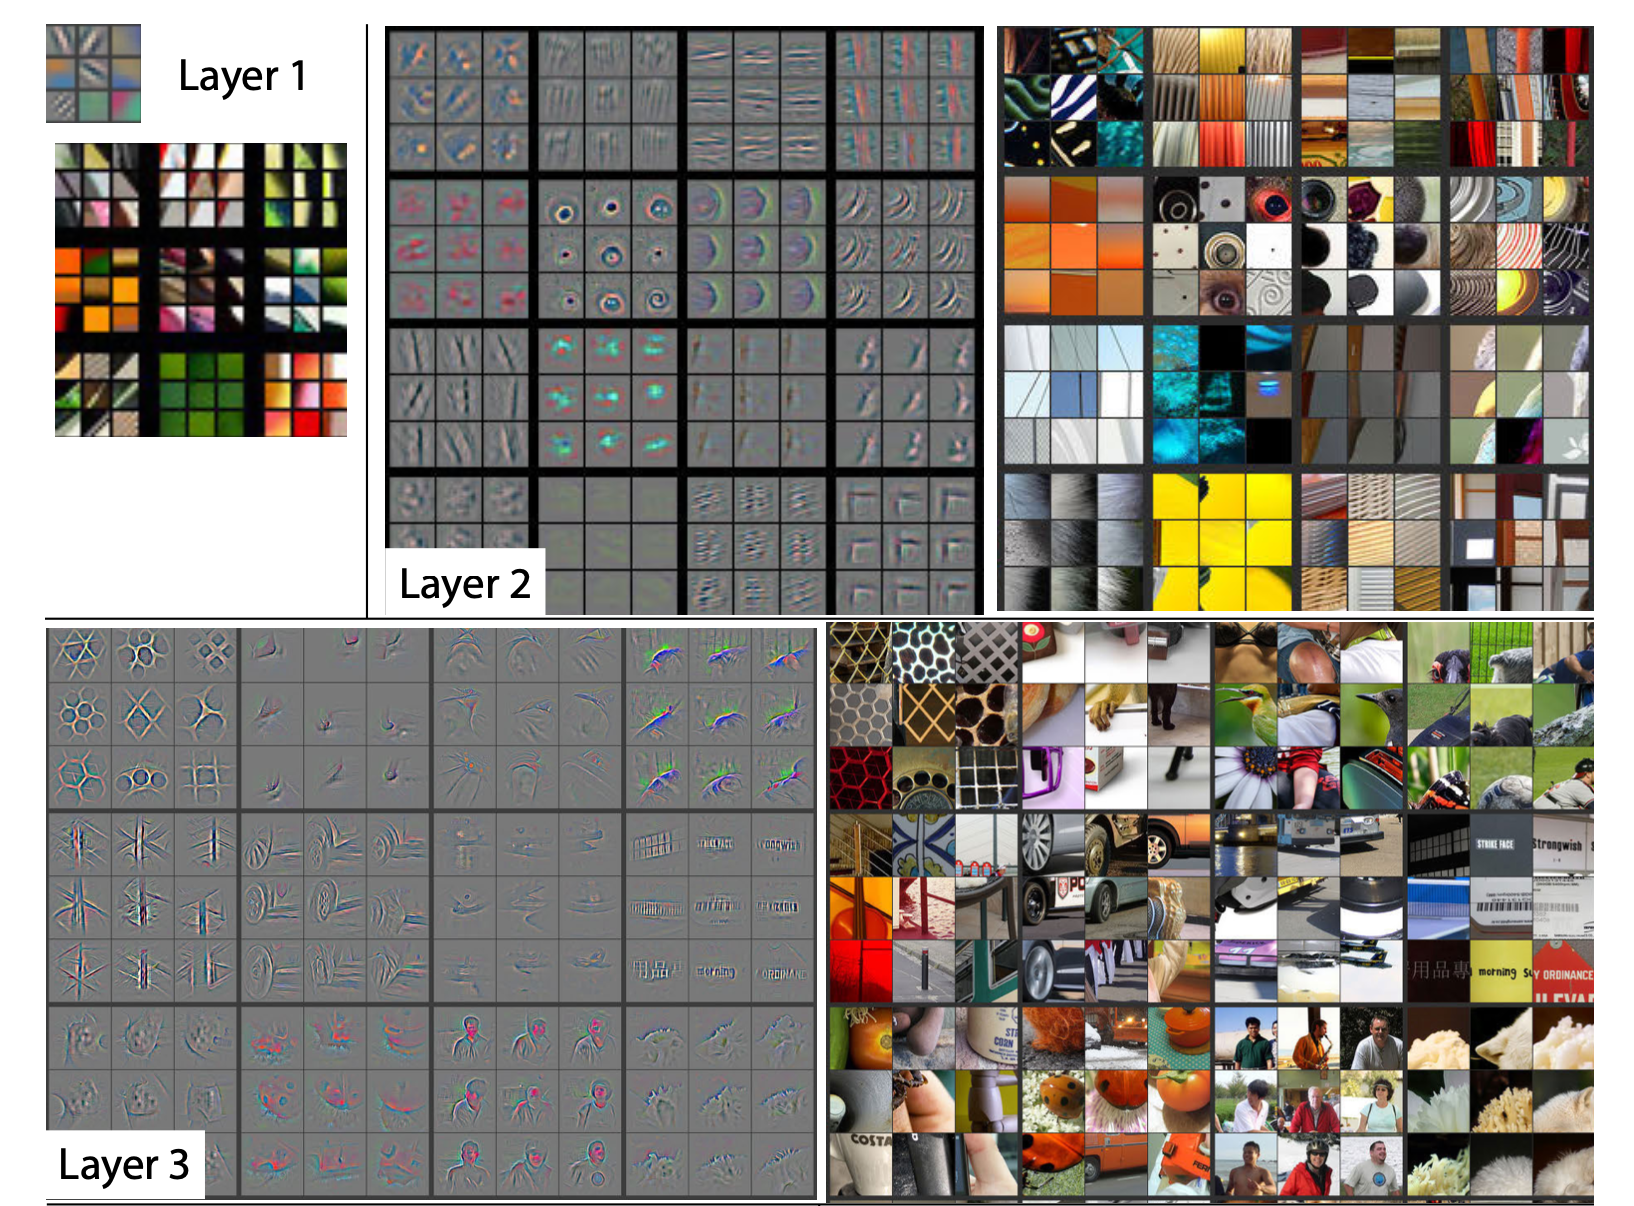
\includegraphics[width=\linewidth]{Zeiler2013-DeconvMaps.png}
    \caption{DeconvNet maps (source: \cite{Zeiler2013})}
    \label{fig:deconvnetmaps}
\end{figure}

\subsection{Saliency maps}
\cite{Erhan2009}, \cite{Simonyan2014}

Saliency map is a visualization technique using gradient-based method to observe the behavior of a deep neural network. We will tackle two different approaches :
\begin{itemize}
    \item Class model visualization
    \item Image-specific class saliency visualization
\end{itemize}  
Then, we will study the link between these techniques and the DeconvNet reconstruction.

With a class model visualization, we generate a picture representing a given class to understand the structure/behavior of it.

Formally, we want to maximize the difference between the score of a given class and our regularized picture : 
\[\arg \underset{I}{\max} {S_c(I)-\lambda{\Vert I \Vert^2}}\]

Furthermore, we use the score of the given class and not the class posterior because it is possible to maximize the previous difference discriminating others classes.

With image-specific class saliency visualization, we want to understand neural contribution/influence on the classification choice.
\begin{itemize}
    \item First, we generate a baseline typically a grey-scale image with a given class \(c\).
    \item Then, after  we find \(w\) by back-propagation.   
    \item Finally, this is how we generate the image : \(M_{(i,j)} = |w_{h(i,j,c)}|\) where \((i,j)\) is pixel position.
\end{itemize}

This method is particularly used for object location. Indeed, the magnitude of \(w\) and the picture profil are linked.

We can compare these methods to DeconvNet reconstruction which is based on back-propagation from the output of the DNN. The derivation keeps linearity and activation functions are approximated. \cite{Simonyan2014} shows that these gradient-based methods are equivalent.

\subsubsection{Enhanced saliency maps}

Images produced by back-propagation look very weird to human, they contain part of objects or artifacts that are repeated. \cite{Mahendran2015} and \cite{Nguyen2016} are making proposals to get saliency images that are more interpretable by humans. When performing the gradient maximization through back-propagation, regularizers are added to avoid high frequency pixel variations and favor the center part of the image.

Moreover, in \cite{Nguyen2016}, the baseline (called there prior) is selected in order to trigger the saliency of several facets of the target neuron. This is performed by computing the activation of many images triggering the target neuron, projecting these activations to 2D with t-SNE and then performing K-means clustering. This technique is used later in \cite{Carter2019}.

\subsection{Integrated gradients}
\cite{Sundararajan2017}

The main issue of any machine learning model is the link between the prediction and the input features. This problem is fundamental with DNN which behaves as black boxes.

\cite{Sundararajan2017} put the two following axioms to answer this problem: 
\begin{itemize}
    \item Sensitivity : \emph{"for every input and baseline that differ in one feature but have different predictions then the differing feature should be given a non-zero attribution"}
    \item Implementation invariance : \emph{"Two networks are functionally equivalent if their outputs are equal for all inputs, despite having very different implementation"}
\end{itemize}

\cite{Sundararajan2017} defines a gradient-based method respecting these two axioms : integrated gradients.

\[IntegratedGrads_i(x) = (x_i - \tilde{x_i}) \int_{\alpha=0}^{1} \frac{\partial F(\tilde{x}+\alpha x (x-\tilde{x}))}{\partial x_i} d\alpha \]

where F is a DNN, x the input et \(\tilde{x}\) the baseline. 

Integrated gradients verifies the following proposition : 

\[\sum_{i=1}^{i=n} IntegratedGrads_i(x) = F(x) - F(x) \]

This approach is interesting by the good results we obtained for instance in object location. Moreover the previous axioms help us to link the contribution of main features of DNN.

\subsection{Activation differences}
\cite{Shrikumar2017}

As for Integrated Gradients (see above), Activation differences is based on the comparison of the test image (or sample) to a baseline in order to find which pixels are the most contributing to the final classification or to any neuron unit activation.

Deep lift is designed in order to compute the \(C_{\Delta_{x_i},\Delta_{t}}\) such that:

\[ \sum_{i=1}^n C_{\Delta_{x_i},\Delta_{t}} = \Delta_t\]

It is computed through a modified chain rule of multipliers.

Let's define a multiplier on the contribution of \(\Delta_x\) to \(\Delta_t\) as : 
\(m_{\Delta_{x},\Delta_{t}} = \frac{C_{\Delta_{x_i},\Delta_{t}}}{\Delta_x} \)

The chain rule of multiplier through an hidden layer of units \(y_i\) is :

\[ m_{\Delta_{x},\Delta_{t}} = \sum_j m_{\Delta_{x},\Delta_{y_j}} m_{\Delta_{y_j},\Delta_{t}}  \]

\begin{figure}
    \centering
    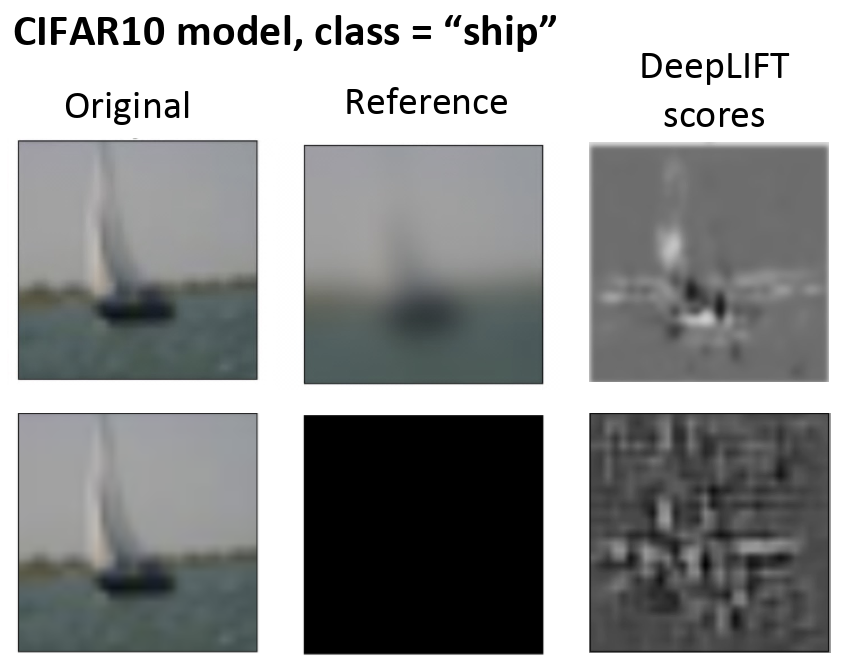
\includegraphics[scale=0.5]{Shrikumar2017-BaselineImportance.png}
    \caption{DeepLIFT on baseline (reference) importance (source: \cite{Shrikumar2017})}
    \label{fig:deeplift-baseline}
\end{figure}

One refinement of the latest paper on DeepLIFT is to separate positive and negative contributions:

\[\begin{aligned} \Delta y &=\Delta y^{+}+\Delta y^{-} \\ C_{\Delta y \Delta t} &=C_{\Delta y^{+} \Delta t}+C_{\Delta y^{-} \Delta t} \end{aligned}\]
 

\subsection{Attribution maps overview and comparison}

\cite{Ancona2018} is performing a review of all the methods explained in this section, and the Layer-wise Relevance Propagation (LRP) of \cite{Bach2015}. We have not reviewed the LRP as it is found to be close to the DeepLIFT but with more limitations.

Conclusions of this paper are:
\begin{itemize}
    \item Integrated gradients are slightly outperforming DeepLIFT since the latter does not support some products of non-linear functions (activations)
    \item All the reviewed techniques are relying on a linear approximation of the network. Their performance is optimum only in case of linear model.
\end{itemize}


\subsection{Map Atlases}

Compared to the original activation maps, saliency and attribution maps are great improvements since they map layer units back to the image space which is interpretable by a human vision. However, the complexity is still high as there are still a huge number of units to visualize and the display is based on an image or a small set if images as in \ref{fig:deconvnetmaps}.

To get a better understanding of the impact of several images and to find similarities of the attribution maps, \cite{Nguyen2016} is using t-SNE in order to group saliency maps with similarities.

\begin{figure}[H]
    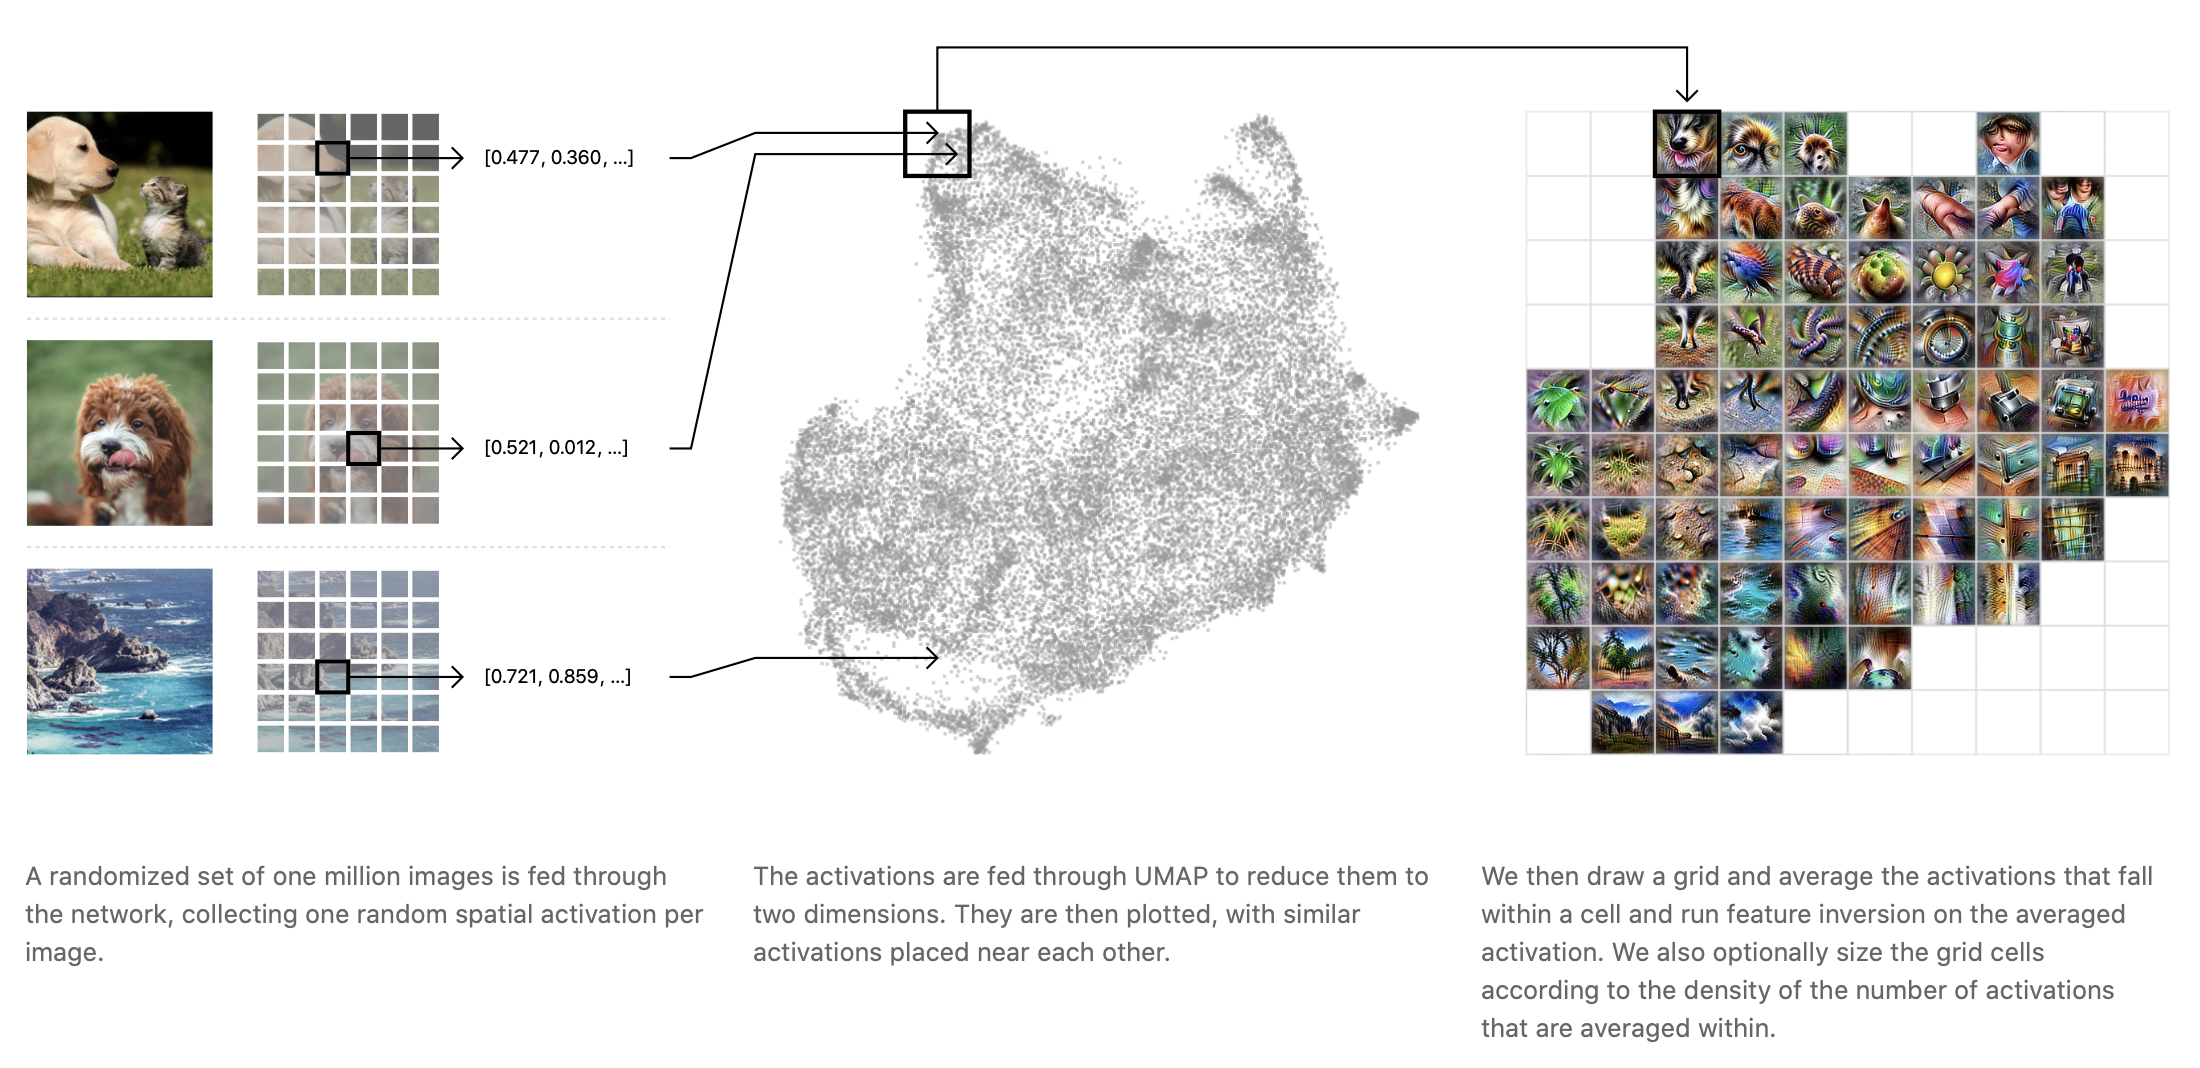
\includegraphics[width=\linewidth]{Carter2019-AtlasHow.png}
    \caption{Activation atlas \cite{Carter2019}, combination of saliency maps}
    \label{fig:atlas-how}
    \centering
\end{figure}

Activation atlases of \cite{Carter2019} goes one step further by sampling activations from many images, using t-SNE or UMAP to gather activation within the 2D plan, and averaging the saliency maps.



